% -*- mode: LaTeX; coding: utf-8 -*-
% Typeset with: XeLaTeX

\documentclass{beamer}
\mode<presentation>
{
  \usetheme[progressbar=foot,numbering=fraction,background=light]{metropolis} 
  \usecolortheme{default} % or try albatross, beaver, crane, ...
  \usefonttheme{default}  % or try serif, structurebold, ...
  \setbeamertemplate{navigation symbols}{}
  \setbeamertemplate{caption}[numbered]
  %\setbeamertemplate{frame footer}{My custom footer}
}
\centering

\usepackage{graphicx}
\graphicspath{ {./figures/} }
\usepackage{hyperref,xcolor}
\newcommand{\link}[2]{\href{#1}{\textcolor{blue}{\underline{#2}}}}

% Main document
\begin{document}
\title{Convergence diagnostics for Markov chain Monte Carlo}
\subtitle{Geometric Data Analysis}
\author{Thomas Pappas}
%\date{4 March 2020}
\maketitle

\begin{frame}{Agenda}
  \tableofcontents[hideallsubsections]
\end{frame}

\section{What are Convergence Diagnostics?}

\begin{frame}{What are Convergence Diagnostics?}
  \begin{block}{}
    Determining convergence of the underlying Markov chain to stationarity and convergence of Monte Carlo estimators to population quantities, respectively.
  \end{block}
  \begin{block}{Answering the following questions}
    \begin{itemize}
      \item When to start the algorithm? ($n^\prime$)
        \begin{itemize}
          \item Remove first results to improve the sample, especially when the initial value is not in a high-density region
          \item Called "burn-in"
        \end{itemize}
      \item When to end the algorithm? ($n^*$) (in relation to the step $\epsilon$)
        \begin{itemize}
          \item Use of $E_\pi g, \bar{g}_{n^\prime,n}$ where $g$ a real-value function of what we need to estimate
        \end{itemize}
      %\item What is the overall convergence assessment of the Markov chain to the stationary distribution?
    \end{itemize}
  \end{block}
\end{frame}

\section{MCMC Diagnostics}

\begin{frame}{Honest MCMC}
  Method for finding $n^\prime$ and $n^*$
  \begin{block}{Honest value for burn-in}
    For a Markov chain estimator $X_n$ and $f_n$ its density, we know that $X_n$ converges in the total variation (TV) norm for $\pi$, i.e.
    \[
      \frac{1}{2}\int_\chi|f_n(x)-\pi(x)|dx \downarrow 0 \textrm{ as } n \rightarrow \infty
    \]
    Therefore we can take an arbitrary cutoff value (here $0.01$) and find the smallest number $n^\prime$ such that
    \[
      \frac{1}{2}\int_\chi|f_{n^\prime}(x)-\pi(x)|dx < 0.01
    \]
    TV norm generally not available, use of \textit{drift} and \textit{minorization} (d\&m) technique to construct a quantitative bound.
  \end{block}
\end{frame}

\begin{frame}{Honest MCMC}
  \begin{block}{Honest stopping rule - Background}
    Let $g$ be a real value function so that $E_\pi g$ becomes a particular feature of the target density. From the strong law of large numbers we get
    \[
      \bar{g}_{n^\prime,n} \equiv \sum_{i=n^\prime}^n g(X_i)/(n-n^\prime) \rightarrow E_\pi g \textrm{ as } n \rightarrow \infty
    \]
    We take $n^\prime = 0$ and we write $\bar{g}_n$ for $\bar{g}_{0,n}$.
  \end{block}
\end{frame}

\begin{frame}{Honest MCMC}
  \begin{block}{Honest way to stop the chain - Background}
    Now if a central limit theorem (CLT) is available for $\bar{g}_n$ , we get
    \[
      \sqrt{n}(\bar{g}_n-E_\pi g) \rightarrow^d N(0,\sigma_g^2) \textrm{ as } n \rightarrow \infty
    \]
    where
    \[
      \sigma_g^2 \equiv Var_\pi(g(X_0))+2\sum_{i=1}^\infty Cov_\pi(g(X_0),g(X_i)) < \infty
    \]
    If $\widehat{\sigma}_{g,n}$ is a consistent estimator of $\sigma_g$, then an estimator of the standard error of $\bar{g}_n$ is $\widehat{\sigma}_{g,n}/\sqrt{n}$.
  \end{block}
\end{frame}

\begin{frame}{Honest MCMC}
  \begin{block}{Honest way to stop the chain - fixed-width stopping rule (FWST)}
    To achieve the confidence interval to fall under a threshold $\epsilon$, we terminate the simulation, first after $\tilde{n}$ iterations, and then when
    \[
      t_*\frac{\widehat{\sigma}_{g,n}}{\sqrt{n}}+\frac{1}{n} \leq \epsilon
    \]
    Note that:
    \begin{itemize}
      \item We execute $\tilde{n}$ iterations to avoid early stop due to poor estimate of $\widehat{\sigma}_{g,n}$
        \begin{itemize}
          \item Value should depend on the complexity of the problem
          \item $\tilde{n} = 10^4$ works well in practice
        \end{itemize}
      \item $t_*$ is an appropriate quantile
        \begin{itemize}
          \item In relation with the confidence interval $100(1-\alpha)\%$
        \end{itemize}
    \end{itemize}
  \end{block}
\end{frame}

\begin{frame}{Graphical methods}
  Methods for MCMC convergence diagnosis
  \begin{block}{Trace plot}
    Time series plat that shows the realisations of the Markov chain at each iteration against the iteration numbers.
    \begin{itemize}
      \item Visualise the movement in the state space
      \item If the chain is "stuck" then it shows flat bits
        \begin{itemize}
          \item e.g. if in Metropolis-Hasting (MH) we have many consecutive rejections or acceptances
        \end{itemize}
    \end{itemize}
  \end{block}
\end{frame}

\begin{frame}{Graphical methods}
  \begin{block}{lag-$k$ autocorrelation}
    The correlation between the samples $k$ steps apart. Shows values of the lag-$k$ autocorrelation function (ACF) against increasing $k$ values.
    \begin{itemize}
      \item For fast-mixing Markov chains, ACF should quickly drop to $0$
    \end{itemize}
  \end{block}
  \begin{block}{Running mean plot}
    Shows the Monte Carlo time average estimates against the iterations.
    \begin{itemize}
      \item Line plot should stabilise to a fixed number
      \item Used to decide stopping times
      \item Has faced criticism
    \end{itemize}
  \end{block}
  %In the multivariant case, all above methods are made by using marginal chains
\end{frame}

%\begin{frame}{Two spectral density-based methods?}
%
%\end{frame}
%
%\begin{frame}{Effective sample size?}
%
%\end{frame}

\section{Examples}

\begin{frame}{An exponential target distribution}
  \begin{block}{}
    \begin{itemize}
      \item Target distribution: $Exp(1)$
      \item Target density: $\pi(x) = exp(-x), x > 0$
      \item Independence Metropolis sampler $Exp(\theta)$
        \begin{itemize}
          \item density: $q(x) = \theta exp(-\theta x), x > 0$
        \end{itemize}
      \item We study the independence chain corresponding to\\
        $\theta = 0.5$ and $\theta = 5$
    \end{itemize}
  \end{block}
\end{frame}

\begin{frame}{An exponential target distribution}
  \begin{block}{Graphical methods}
    \begin{itemize}
      \item We run for 1,000 iterations
      \item $X_0 = 0.1$
    \end{itemize}
  \end{block}
\end{frame}

\begin{frame}{An exponential target distribution}
  \begin{block}{Trace and autocorrelation plots}
    \begin{figure}[h]
      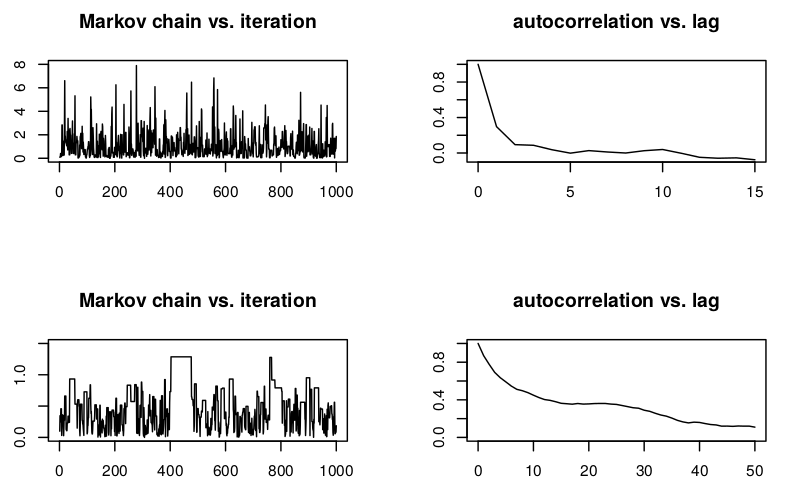
\includegraphics[width=0.8\textwidth]{example1_trace_autocorrellation_plot}
      \caption{Trace and autocorrelation function plots. Top row, $\theta = 0.5$; bottom row, $\theta = 5$.}
    \end{figure}
  \end{block}
\end{frame}

\begin{frame}{An exponential target distribution}
  \begin{block}{Trace and autocorrelation plots}
    \begin{itemize}
      \item For $\theta = 0.5$ the chain mixes well but for $\theta = 5$ the chain needs to be run longer
      \item $\theta = 0.5$ seems to require no burn-in in contrast with $\theta = 5$
    \end{itemize}
  \end{block}
\end{frame}

\begin{frame}{An exponential target distribution}
  \begin{block}{Honest burn-in}
    For $\theta < 1$, we get that
    \[
      \pi(x) / q(x) = \theta^{-1}exp(x(\theta-1)) \leq \theta^{-1}, x > 0
    \]
    and therefore (according to Mengersen and Tweedie (1996))
    \[
      \frac{1}{2}\int_{\chi}|f_n(x)-\pi(x)|dx \leq (1-\theta)^n
    \]
    which is an analytical upper bound of the TV norm. So for $\theta = 0.5$ if $n^\prime = \lceil log(0.01)/log(0.5)\rceil = 7$ can be an appropriate burn-in.\\
    For $\theta = 5$ the upper bound can't be used.
  \end{block}
  % For $\theta = 5$ the independence chain becomes subgeometric and...
\end{frame}

\begin{frame}{An exponential target distribution}
  \begin{block}{Honest way to stop the chain}
    We consider estimation of the mean of the stationary distribution, i.e. $E_\pi X = 1$.
    \begin{itemize}
      \item We apply FWSR for $\epsilon = 0.005$ and $\alpha = 0.05$
        \begin{itemize}
          \item Which makes $t_* = 1.96$
        \end{itemize}
    \end{itemize}
    \begin{itemize}
      \item For $\theta = 0.5$
        \begin{itemize}
          \item Starting at $X_s = 0.1545$
          \item $n^* = 323,693$ iterations
        \end{itemize}
      \item For $\theta = 5$
        \begin{itemize}
          \item Starting at $X_0 = 0.1$
          \item $n^* = 323,700$ iterations
          \item No CLT function available so can't compute asymptotic confidence intervals
        \end{itemize}
    \end{itemize}
  \end{block}
\end{frame}

\begin{frame}{An exponential target distribution}
We run mean estimates to evaluate the results
  \begin{figure}[h]
    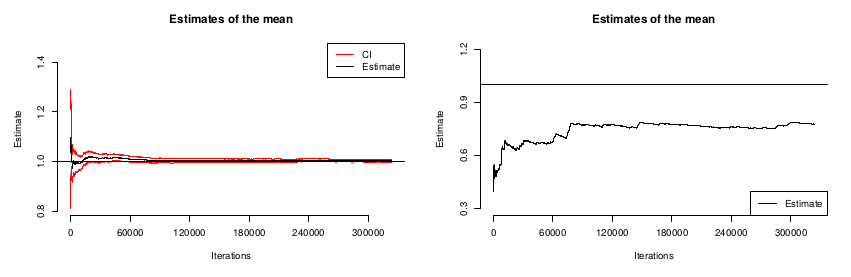
\includegraphics[width=1\textwidth]{example1_mean_estimates}
    \caption{Running mean estimates, on the left for $\theta = 0.5$ with confidence intervals, on the right for $\theta = 5$ without. The horizontal line denotes the truth.}
  \end{figure}
  Conclusions are the same as before
\end{frame}

%\begin{frame}{A Bayesian logistic model?}
%
%\end{frame}

\begin{frame}{Contact details}
  \begin{center}
    Thomas Pappas\\
    \link{mailto:thpappas@di.uoa.gr}{thpappas@di.uoa.gr}
  \end{center}
\end{frame}

\end{document}
